% A sample document for testing. Both its content and its figures are fictitious, made up for the tests.
\documentclass[10pt,twocolumn]{article}
\usepackage[a4paper,margin=18mm,columnsep=7mm]{geometry}
\usepackage[T1]{fontenc}
\usepackage{lmodern}
\usepackage{amsmath,booktabs,xcolor,tikz,caption,enumitem}
\setlist{nosep,leftmargin=1.4em}
\pagestyle{plain}

\title{\bfseries Layout-Preserving Translation of PDF Documents\\ inside a Code Editor}
\author{Alex Example \and Sam Sample\\[2pt] \small Institute of Document Engineering}
\date{}

\begin{document}
\twocolumn[
  \maketitle
  \vspace{-7mm}
  \begin{center}
  \colorbox{blue!9}{\parbox{0.88\textwidth}{\vspace{2mm}\small\textbf{Abstract.}
  We describe a viewer that shows a PDF document and its translation side by side
  without changing the design of the page. The page is drawn twice by the same
  rendering engine, once as it is and once without text, and the translated text is
  placed over the second drawing. Figures, rules, and coloured backgrounds therefore
  stay exactly as they are in the source. The translation is produced block by block,
  so the reader sees the first paragraphs after a few seconds.\vspace{2mm}}}
  \end{center}
  \vspace{5mm}
]

\section{Introduction}
Reading technical documents in a second language is slow, and switching between a
viewer and a translation tool breaks concentration. Many readers therefore want the
translation to appear next to the original, in the same position on the page, so that
figures, tables, and equations can still be found at a
glance.\footnote{This is a synthetic sample document made for testing. All numbers in it are invented.}

Existing tools usually follow one of two routes. The first converts the document to
plain text or HTML and translates the result; this is simple, but the original design
is lost. The second rebuilds a new PDF file with translated text; this keeps the
design, but it needs a heavy pipeline, and the reader must wait until the whole file is
finished~[1, 2].

In this paper we take a third route. The page is drawn twice by the same rendering
engine: once as it is, and once without any text. The translated text is then placed
over the second image as ordinary web content. Because everything except the text
comes from the original drawing commands, backgrounds, rules, and figures are
identical to the source.

Our contributions are as follows:
\begin{itemize}
\item a rendering scheme that removes text without touching vector graphics or images;
\item a simple geometric method for grouping text into paragraphs;
\item a fitting procedure that keeps each translated paragraph inside its original box.
\end{itemize}

\section{Method}
\subsection{Text-free rendering}
A PDF page is a list of drawing operators. Let $P = (o_1, \dots, o_n)$ be this list and
let $T \subset P$ be the operators that show text. We render the full list to obtain an
image $I_{\mathrm{full}}$ and the filtered list $P \setminus T$ to obtain
$I_{\mathrm{bare}}$. For a translated region $R$ the displayed image is
\begin{equation}
I(x) =
\begin{cases}
I_{\mathrm{bare}}(x) & x \in R,\\
I_{\mathrm{full}}(x) & \text{otherwise.}
\end{cases}
\end{equation}
Regions that are not translated, such as equations and labels inside figures, keep
their original pixels.

\subsection{Block segmentation}
Text fragments are first merged into lines by comparing baselines, and lines are then
merged into blocks when they share a font size, overlap horizontally, and follow the
regular line pitch of the page. A new block starts at an indented line, at a list
marker, or after a vertical gap.

\subsection{Fitting the translation}
Japanese text often needs slightly more room than English. For each block we search
for the largest scale $k \in [0.7, 1]$ such that the translated paragraph does not
exceed the height of the original box. If no such scale exists, the paragraph may
extend into the empty space below it.

\medskip
\noindent\colorbox{black!82}{\parbox{\dimexpr\columnwidth-2\fboxsep}{\color{white}\small
\textbf{Note.} The source file is never modified. Closing the translated view returns
the reader to the original document.}}

\section{Experiments}
We measured the method on 120 pages taken from manuals, reports, and research papers.
Table~1 shows the share of blocks that fitted into their original boxes, and Figure~1
shows how the time to the first translated block changes with the length of the page.

\begin{table}[t]
\centering\small
\caption{Share of translated blocks that fit into the original box.}
\begin{tabular}{lrrr}
\toprule
Document type & Pages & Blocks & Fit (\%)\\
\midrule
Manuals & 40 & 1,120 & 96.4\\
Reports & 40 & 980 & 93.1\\
Research papers & 40 & 1,460 & 89.7\\
\bottomrule
\end{tabular}
\end{table}

\begin{figure}[t]
\centering
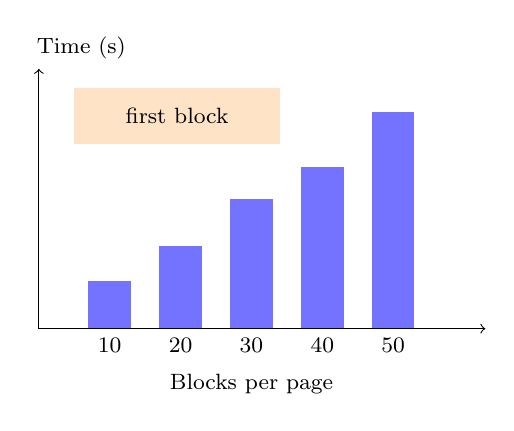
\begin{tikzpicture}[x=9mm,y=0.5mm]
  \fill[orange!22] (0.5,47) rectangle (3.4,61);
  \node at (1.95,54) {\footnotesize first block};
  \foreach \x/\h/\l in {1/12/10,2/21/20,3/33/30,4/41/40,5/55/50} {
    \fill[blue!55] (\x-0.3,0) rectangle (\x+0.3,\h);
    \node[below] at (\x,0) {\footnotesize \l};
  }
  \draw[->] (0,0) -- (6.3,0);
  \draw[->] (0,0) -- (0,66);
  \node[below] at (3,-9) {\footnotesize Blocks per page};
  \node[above] at (0.6,66) {\footnotesize Time (s)};
\end{tikzpicture}
\caption{Time until the first translated block appears.}
\end{figure}

The share is lowest for research papers, because their pages are dense and leave
little empty space below each paragraph.

\section{Limitations}
Scanned pages contain no text operators, so they need optical character recognition
before translation. Tables are translated cell by cell, which can break sentences that
span several cells. Inline mathematics is sent to the model as plain text and may be
altered.

\section{Conclusion}
Drawing the page twice and overlaying translated text keeps the design of the original
document while remaining light enough to run inside an editor. We plan to add support
for exporting the result as a new PDF file.

\begin{thebibliography}{9}\small
\bibitem{a} A.~Example and S.~Sample. Rebuilding translated documents from an
intermediate representation. \emph{Journal of Document Engineering}, 12(3):45--67, 2024.
\bibitem{b} C.~Placeholder. A survey of layout analysis for born-digital documents. In
\emph{Proceedings of the Workshop on Document Layout}, pages 1--10, 2025.
\end{thebibliography}

\end{document}
